\section{Debugger Testing DSL}

\emph{DeTeL} is integrated in \ic{MPS} and interacts
with mbeddr's debugger \ic{API}. While this language is currently tightly
coupled to mbeddr, it could in theory interact with a generic debugger \ic{API}
and be implemented with a language workbench other than \ac{MPS}.
This section describes the structure of \emph{DeTeL} and the
implementation of design decisions discussed in \sect{DesignDecisions}.

\subsection{DebuggerTest}

\fig{fig:DebuggerTestStructure}) shows the structure of 
\ic{DebuggerTest}, which is a module that \emph{contains} 
\ic{ITestContent}s, currently implemented by 
\ic{DebuggerTestcase} and \ic{CallStack} (described later). This interface
facilitates extensibility inside
\ic{DebuggerTest} (\hyperref[O2]{O2}). Further, \ic{DebuggerTest} refers to 
a \ic{Binary} (concept from mbeddr representing the compiled mbeddr program
under test, \hyperref[R3]{R3}), \emph{imports} of \ic{ITestContent}s from other 
\ic{DebuggerTest}s (\hyperref[O1]{O1}) and an
\ic{IDebuggerBackend} that specifies the debugger backend to use
(\hyperref[O2]{O2}, \hyperref[M1]{M1}). Latter is implemented by
\ic{GdbBackend} and allows this way to run debugger tests with the
\ac{GDB}~\cite{gdb}.

\begin{figure}[h]
  \vspace{-2mm}
  \centering
    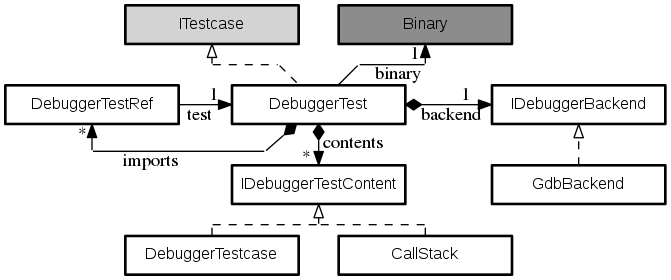
\includegraphics[width=8.5cm]{./figures/graph2-1.png} 
    \vspace{-2mm}
    \caption{\ic{DebuggerTest} structure: \emph{DeTeL} concepts 
    (white boxes), \ic{ITest- case} (light gray box) is from
    \ac{MPS} and \ic{Binary} (dark grey box) from mbeddr.}
  \label{fig:DebuggerTestStructure}
  \vspace{-2mm}
\end{figure}

\ac{MPS} comes already with the language \ic{mps.lang.test} for writing type
system and editor tests. Its \ac{MPS} integration allows users to (1) execute
tests \emph{automatically} (on the command-line and inside the \ac{IDE}) and 
(2) get the results of
executed tests visualized in a table view. All of that functionality is build
for implementations of \ic{ITestcase} - an interface from \ic{mps.lang.test}. By
implementing this interface in \ic{DebuggerTest} (our container for
\ic{DebuggerTestcase}s), we get the \ic{IDE} integration and the ability to
run our tests \emph{automatically} (\hyperref[O3]{O3}).



\subsection{CallStack}

\ic{CallStack} implements \ic{ITestContent} 
(see \fig{fig:CallStackStructure}) and contains
\ic{IStackFrame}s (\hyperref[O2]{O2}, \hyperref[R1]{R1}). Each frame
specifies a \emph{name}, visible \emph{watches} and the \emph{location} where suspended.
We have two implementations of \ic{IStackFrame}:
\ic{StackFrame} and \ic{StackFrameExtension}.
While an \emph{extend}ing \ic{CallStack} can declare additional
\ic{StackFrame}s, it contains for each inherited
\ic{StackFrame} a \ic{StackFrameExtension} that allows specialization of
inherited properties (\hyperref[O1]{O1}).

\begin{figure}[h]
  \vspace{-2mm}
  \centering
    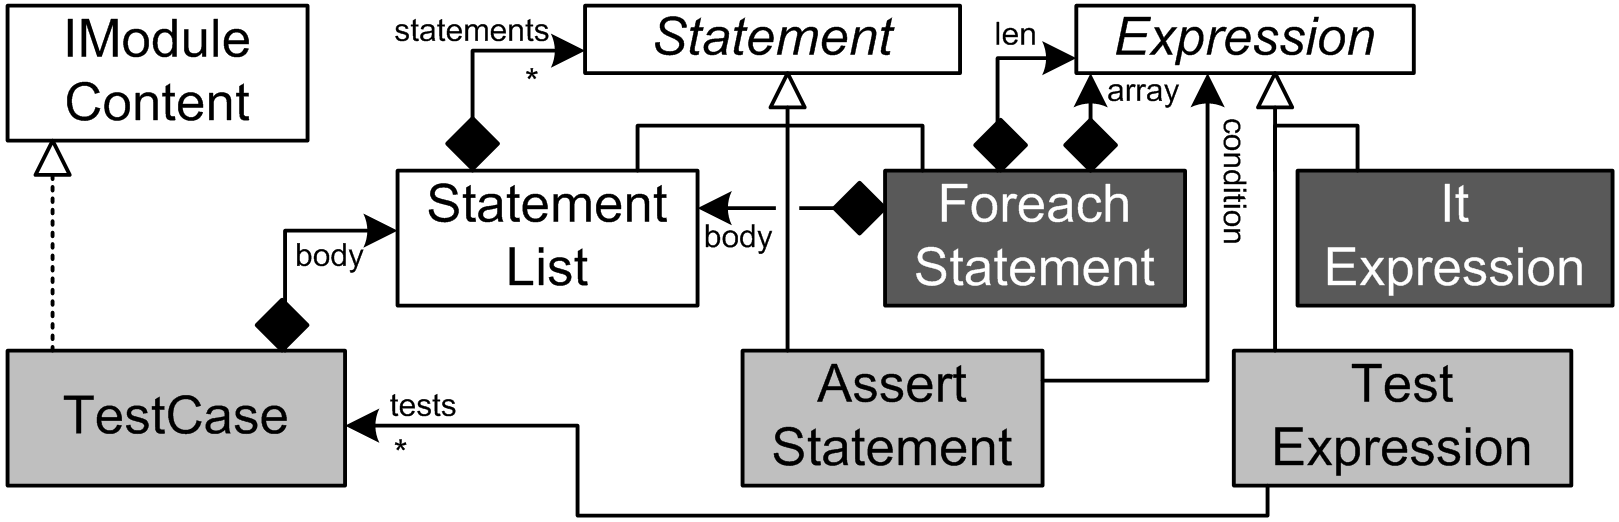
\includegraphics[width=8.5cm]{./figures/umldiag.png} 
    \vspace{-2mm}
    \caption{Structure of \ic{CallStack}s}
  \label{fig:CallStackStructure}
  \vspace{-2mm}
\end{figure}

\ic{IStackFrame} has three parts: a \emph{name} 
(\ic{IStackFrameName}), a location where execution should suspend
(\ic{ISuspend- Location}) and visible watches (\ic{IWatches}).

\ic{IName} has two implementations: while \ic{SpecificName} verifies
a specific \emph{name}, \ic{AnyName} ignores the \emph{name}.
Next, \ic{ILocation} with its implementations:
\ic{AnyLocation} again does no validations, 
while \ic{ProgramMarkerRef} references a \ic{ProgramMarker}  that represents a
specific location in a program under test (\hyperref[R3]{R3}). Those markers do
not influence code generation, they just annotate nodes in the \ac{AST}.
\ic{IWatches} has two implementations: \ic{AnyWatches} and \ic{WatchList}.
First performs no validations, while the other one holds a list of \ic{Watch}es 
that specify a \emph{name} and a \emph{value} expressed with 
\ic{IValue}. For verifying values, \ic{PrimitiveValue}  (\eg numbers)
or \ic{ComplexValue} (\eg arrays) is used.

\subsection{DebuggerTestcase}

\fig{fig:DebuggerTestcaseStructure} shows the structure of
\ic{DebuggerTestcase}:
can \emph{extend} other \ic{DebuggerTestcase}s (\hyperref[O1]{O1}), specifies a
\emph{name}, and can be \ic{abstract}. Further it holds the following parts:
\ic{SuspendConfig}, \ic{SteppingConfig} and
\ic{Validation- Config}. Concrete \ic{DebuggerTestcase}s require at least  
a \ic{SuspendConfig} and a \ic{ValidationConfig} (can be inherited),
while an \ic{abstract} \ic{DebuggerTestcase} requires none.
 
\begin{figure}[h]
  \vspace{-2mm}
  \centering
    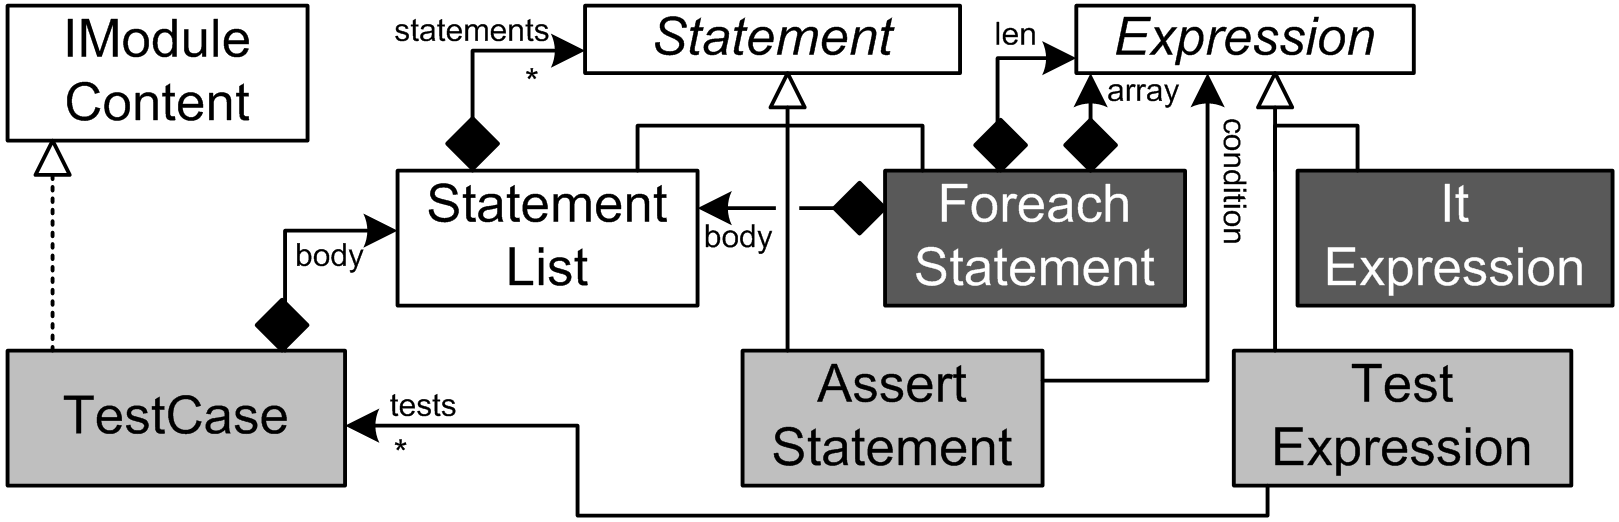
\includegraphics[width=8.5cm]{./figures/umldiag.png} 
    \vspace{-2mm}
    \caption{Structure of \ic{DebuggerTestcase}s}
  \label{fig:DebuggerTestcaseStructure}
  \vspace{-2mm}
\end{figure}

\ic{SuspendConfig} contains a \ic{ProgramMarkerRef} that points to
\emph{location} inside the mbeddr program under tests (\hyperref[R2]{R2}). 
After starting the test, execution first suspends at this \emph{location}. 

\ic{SteppingConfig} is optional and contains a
list of \ic{IStep- pingCommand}s (\hyperref[O2]{O2})that are executed after
suspending on \emph{location} (\hyperref[R2]{R2}). This interface is implemented by 
\ic{StepInto}, \ic{StepOver}, \ic{StepOut} (each performs the command
\emph{n times}). Additionally, \ic{Super} implements the interface, so
the inherited \ic{SteppingConfig} can be extended.

\ic{ValidationConfig} contains a list of \ic{IValidation}s
(\hyperref[O2]{O2}, \hyperref[R1]{R1}), implemented by the previously described
\ic{CallStack}, \ic{CallStackRef}, \ic{OnPlatform} and \ic{Super}. 
While \ic{Super} represents inherited \ic{IValidation}s,
\ic{CallStackRef} refers to a \ic{CallStack} without having the
possibility to modify it.
Finally, \ic{OnPlatform} specifies a \ic{Platform} (\emph{Mac}, \emph{Unix} or
\emph{Windows}) and executes contained \ic{Validation}s only if tests are
executed on that specific \ic{Platform} (\hyperref[R1]{R1}).

\section{Testing the Debugger Extension}

The previously described debugger testing \ac{DSL} is used in this section for
testing the debugger extension of unit testing. While those
tests do not aim for full test coverage, they concentrate on the essential
scenarios to test.

Before writing tests, the program using the unit testing
language from \lst{lst:generatedUT} is annotated with markers
(see listing below). Those markers do not influence the code generation,
however, they are used by \ic{DebuggerTestcase}s to refer to code locations
for specifying where to suspend execution and for verifying where
execution suspended.

\begin{lstlisting}[language=markerDSL]
int32 main(int32 argc, string$[$ $]$ argv) {
   [return test$[$forTest$]$;] onReturnInMain
}
testcase forTest {
   [int32 sum = 0;] onSumVarDeclaration
   [assert: sum == 0;] on1stAssertInTestcase
   [int32$[$ $]$ nums = {1, 2, 3};] onNumsVarDeclaration
   for(int32_t i=0;i<3;i++) { sum += nums[i]; }
   [assert: sum == 6;] onLastStmntInTestcase
}
\end{lstlisting}	

Next, in the listing below an empty \ic{DebuggerTest} \emph{UnitTesting} is
created that will later contain all \ic{Debugger- Testcase}s described in this
section. \emph{UnitTesting} tests against the binary \emph{UnitTestingBinary},
which is compiled from \lst{lst:generatedUT} and further tells the mbeddr
debugger runtime to execute tests with the \ic{gdb} debugger backend.

\begin{lstlisting}[language=testingDSL]
DebuggerTest UnitTesting    tests binary: UnitTestingBinary {
                            uses debugger: gdb

}  
\end{lstlisting}

\subsection{Step Into ExecuteTestExpression}

For testing \emph{step into} on instances of \ic{Execute- TestExpression},
in the listing below a \ic{CallStackDec- laration} is created that specifies how
the stack must be organized after performing \emph{step
into} on \emph{onReturnInMain}. To reuse information and 
minimize redundance in later
\ic{DebuggerTestcase}s, two separate 
\ic{CallStack}s are created: First, \emph{inMain} 
has a single \ic{StackFrame} that expects (1) execution to suspend at  
\emph{onReturnInMain} and (2) two watches to exist (\emph{argc} and
\emph{argv}). Second, \emph{inTestcase} extends
\emph{inMain} by declaring on top of \emph{main} an addition
\ic{StackFrame} \emph{forTest}, which specifies no location, but two
watches (\emph{sum} and \emph{nums}). In \emph{inTestcase}, inherited
\ic{StackFrame}s are colored in gray and not editable, since they are
just a projection of the original.

\begin{lstlisting}[language=testingDSL]
call stack inMain {
   0:main
      location: onReturnInMain
      watches: {argc, argv}                     
}
   
call stack inTestcase extends inMain {
   1:forTest
      location: <any>
      watches: {sum, nums}                  
   $\gT{0}$$\gT{:}$$\gT{main}$
}
\end{lstlisting}

After declaring both \ic{CallStack}s, the listing below contains
the \ic{DebuggerTestcase} \emph{stepIntoTestcase}, which uses \emph{inTestcase}
to verify \emph{step into} for instances of \ic{ExecuteTestExpression}: First,
execution is suspended at \emph{onReturnInMain}, next, a single \emph{step into}
is performed before the actual call stack is validated against
a custom \ic{CallStack} derived from \emph{inTestcase}.
This custom declaration specializes in
\emph{forTest} the expected location to suspend execution with
\emph{onSumDeclaration}.

\begin{lstlisting}[language=testingDSL]
testcase stepIntoTestcase {            
   suspend at: 
      onReturnInMain
   then perform:                         
      step into 1 times    
   finally validate:                         
      call stack stepIntoTestcase extends inTestcase {
         $\gT{1}$$\gT{:}$$\gT{forTest}$
            overwrite location: onSumDeclaration
            $\gT{watches}$$\gT{:}$ $\gT{\{}$$\gT{sum, nums}$$\gT{\}}$
         $\gT{0}$$\gT{:}$$\gT{main}$                       
      }
}
\end{lstlisting}

\subsection{Step into/over AssertStatement}

After verifying \emph{step into} for \ic{ExecuteTestExpression}, 
\emph{step into} and \emph{over} for instances of \ic{AssertStatement} is tested
next. Both step commands have the same outcome when performed at
\emph{1stAssert}, hence common test behavior is extracted into the
\emph{abstract} \ic{DebuggerTestcase} \emph{stepOnAssert} shown below: (1) 
execution suspends on \emph{1stAssert} and a custom \ic{CallStack} verifies 
execution in \emph{forTest} is (2) suspended on \emph{onArrayDecl} and
(3) watch \emph{num} has the value zero.
 
\begin{lstlisting}[language=testingDSL]
abstract testcase stepOnAssert {
   suspend at: 
      1stAssert
   finally validate:
      call stack stepOnAssert extends inTestcase {
         1:forTest
            overwrite location:   onArrayDecl
            overwrite watches: {sum=0,nums}
         0:main                      
      }
}
\end{lstlisting}

While the first \ic{DebuggerTestcase} \emph{stepIntoAssert} extending
\emph{stepOnAssert} performs a \emph{step into}, the other one
\emph{stepOverAssert} performs a \emph{step over}:

\begin{lstlisting}[language=testingDSL]
testcase stepIntoAssert extends stepOnAssert {            
   then perform:                         
      step into 1 times                            
}
testcase stepOverAssert extends stepOnAssert {            
   then perform:                         
      step over 1 times                            
}
\end{lstlisting}

\subsection{Step on last Statement in Testcase}

The last testing scenario verifies that stepping on the last \ic{Statement}
(\emph{2ndAssert}) inside a \ic{Testcase} suspends execution on the caller
\ic{ExecuteTestExpression} (\emph{onReturnInMain}).
The approach for testing this scenario is similar as before (see listing
below): an \emph{abstract} \ic{DebuggerTestcase}
\emph{steppingOnLastStmnt} suspends execution on
\emph{2ndAssert} and verifies the actual call stack has the same structure as
\emph{inMain}.

\begin{lstlisting}[language=testingDSL]
abstract testcase steppingOnLastStmnt {
   suspend at: 
      2ndAssert
   finally validate:
      call stack inMain
}
\end{lstlisting}

Next, for \emph{step over}, \emph{into} and \emph{out} separate
\ic{DebuggerTest- case}s are created, which extend \emph{steppingOnLastStmnt}
and specify the respective stepping command:

\begin{lstlisting}[language=testingDSL]
testcase stepOverLastStmnt extends steppingOnLastStmnt {            
   then perform:                         
      step over 1 times                            
}
testcase stepIntoLastStmnt extends steppingOnLastStmnt {            
   then perform:                         
      step into 1 times                            
}
testcase stepOutFromLastStmnt extends steppingOnLastStmnt {            
   then perform:                         
      step out 1 times                            
}
\end{lstlisting}		
			
	